\section{Fault Trees}

\subsection{Static Fault Trees}

\begin{frame}
\frametitle{Static Fault Trees}
\begin{tikzpicture}[fault tree, global scale=0.7]
\node (r) [event] {Low Power}
    child {
      node (both) [event] {Both inputs fail}
      child { node (a1) [event] {A fails} } 
      child { node (b1) [event] {B fails} }
    }
    child {
      node (si) [event] {One input fails and the switcher fails}
      child { node (s) [event] {Switcher fails}}
      child { 
        node (oneinput) [event] {One input fails}
        child { node (a2) [event] {A fails} }
        child { node (b2) [event] {B fails} }
      }
    };

\node [or gate] (or1) at (r.south) {};
\node [and gate] (and1) at (both.south) {};
\node [and gate] at (si.south) {};
\node [or gate] at (oneinput.south) {};
\node [basic] at (a1.south) {};
\node [basic] at (a2.south) {};
\node [basic] at (b1.south) {};
\node [basic] at (b2.south) {};

\onslide<2->{
\node (rdescr) [above right=0.5cm and 0cm of r] {Root event};
\draw (rdescr) edge[->] (r);

\node (interdescr) [above right=0.5cm and 0cm of si] {Intermediary event};
\draw (interdescr) edge[->] (si);

\node (ordescr) [below right=0 and 0.5cm of or1] {OR gate};
\draw (ordescr) edge[->] (or1);

\node (anddescr) [below right=0 and 0.5cm of and1] {AND gate};
\draw (anddescr) edge[->] (and1);

\node (basicdescr) [below right=0.3 and 0.5cm of a1] {Basic event};
\draw (basicdescr) edge[->] (a1);
}

      %child {
      %  node [and gate] {}
      %  child {
      %    node [event] {One input fails and the switcher fails}
      %    child { node [basic] {Switcher fails} }
      %    child {
      %      node [event] {One input fails}
      %      child {
      %        node [or gate] {}
      %        child [basic] {A fails}
      %        child [basic] {B fails}
      %      }
      %    }
      %  }
      %}
\end{tikzpicture}
\end{frame}

\subsection{Dynamic Fault Trees}

\begin{frame}
\frametitle{Dynamic Fault Trees}
\begin{itemize}
  \item Priority AND -- PAND\\
    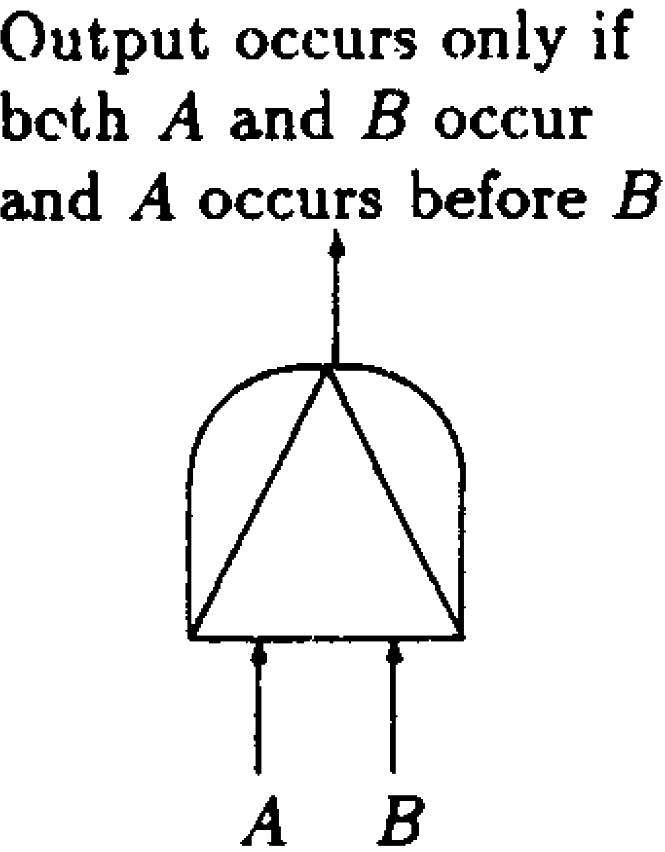
\includegraphics[height=4cm]{pand-dugan}
\end{itemize}
\end{frame}

\begin{frame}
\frametitle{Dynamic Fault Trees}
\begin{itemize}
  \item Cold Spare gate -- CSP\\
    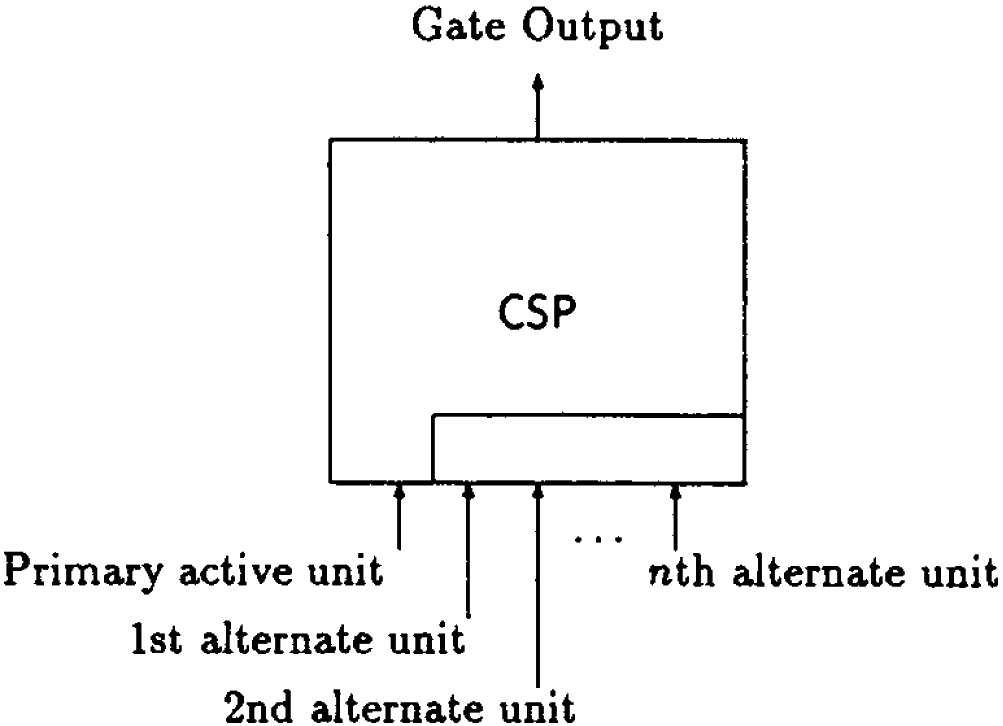
\includegraphics[height=4cm]{csp-dugan}
  \item Example: 4 tires, 1 spare
\end{itemize}
\end{frame}

\begin{frame}
\frametitle{Dynamic Fault Trees}
\begin{itemize}
  \item Sequence Enforcing gate -- SEQ (dummy output)\\
    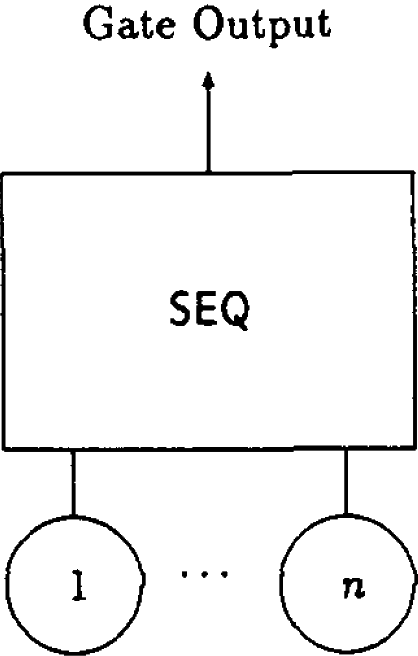
\includegraphics[height=4cm]{seq-dugan} 
  \item Events are forced to occur in a specific order
\end{itemize}
\end{frame}

\begin{frame}
\frametitle{Dynamic Fault Trees}
\begin{itemize}
  \item Functional Dependency gate -- FDEP (dummy output)\\
    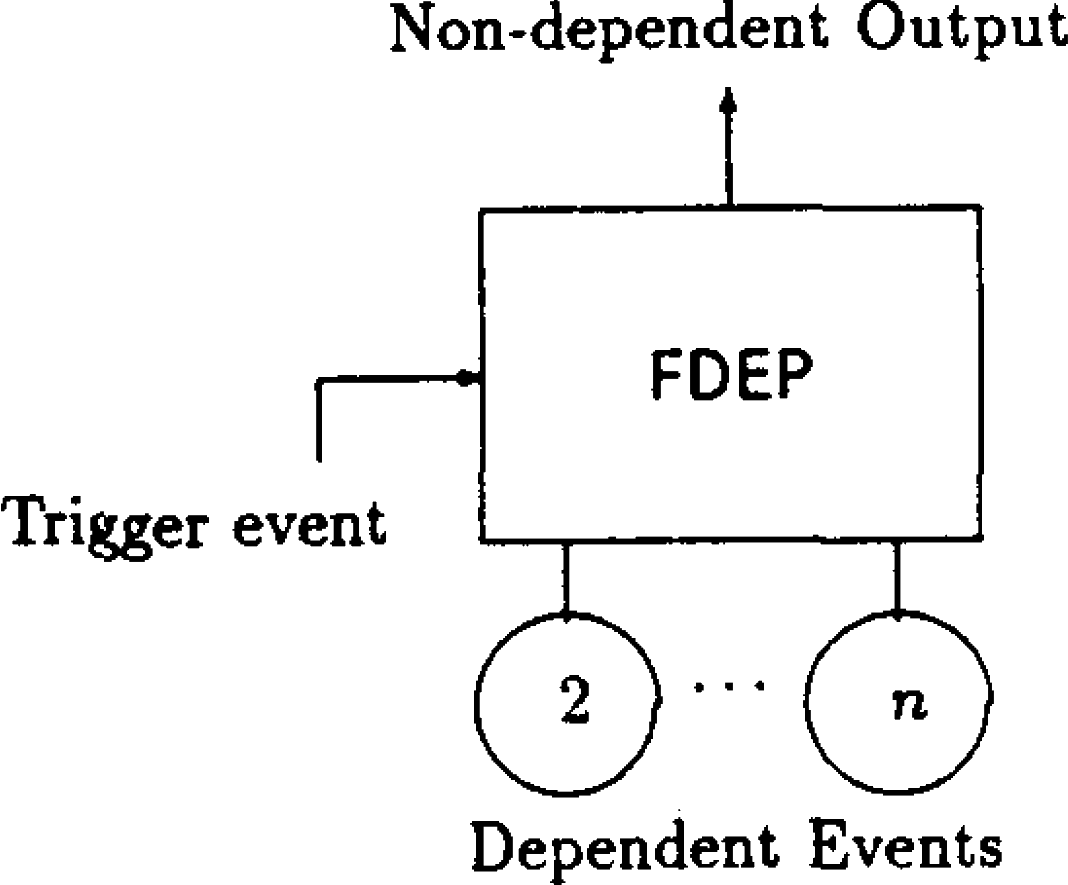
\includegraphics[height=4cm]{fdep-dugan}
  \item Dependent events are forced to occur when the trigger events activates;
  \item Otherwise they are independent.
\end{itemize}
\end{frame}

\begin{frame}
\frametitle{Relevant DFT gates}
\begin{itemize}
  \item SEQ is expressible in terms of CSP.
  \item For DFT, the relevant gates are then PAND, FDEP and CSP. 
\end{itemize}
\end{frame}

\subsection{Temporal Fault Trees}

\begin{frame}
\frametitle{Temporal Fault Trees}
\begin{itemize}
  \item Priority AND gate -- PAND\\
  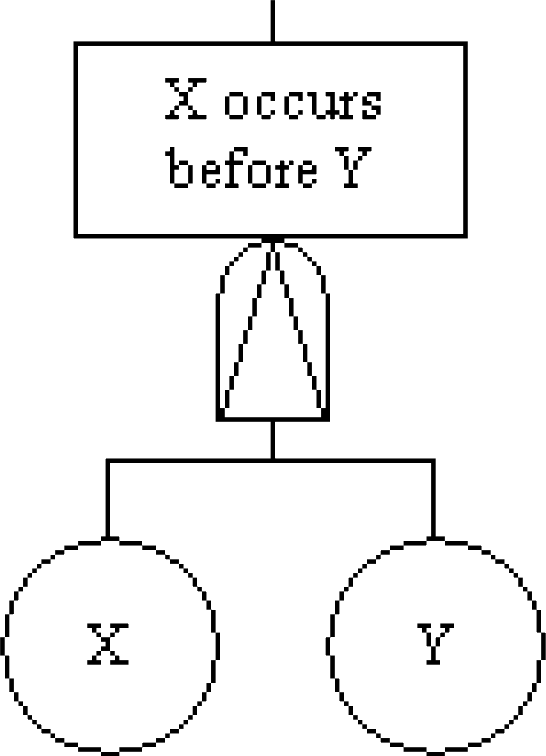
\includegraphics[height=4cm]{pand-walker}
\end{itemize}
\end{frame}

\begin{frame}
\frametitle{Temporal Fault Trees}
\begin{itemize}
  \item Priority OR gate -- POR\\
  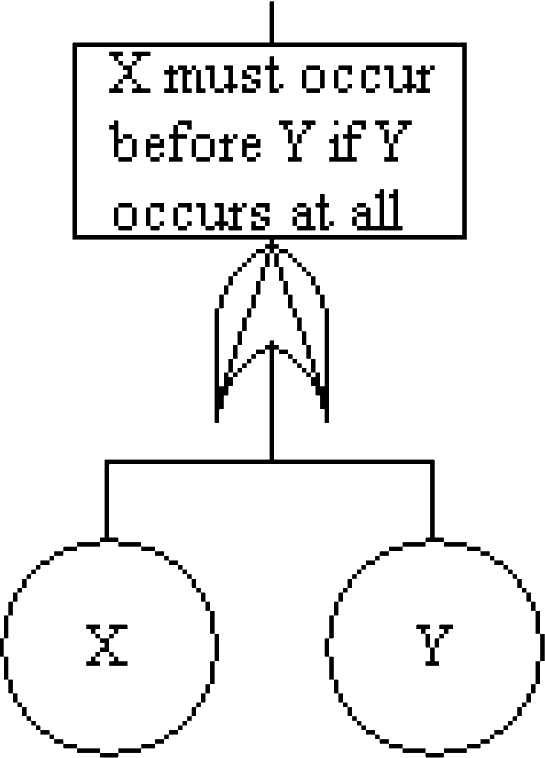
\includegraphics[height=4cm]{por-walker}
\end{itemize}
\end{frame}

\begin{frame}
\frametitle{Temporal Fault Trees}
\begin{itemize}
  \item Simultaneous gate -- SAND\\
  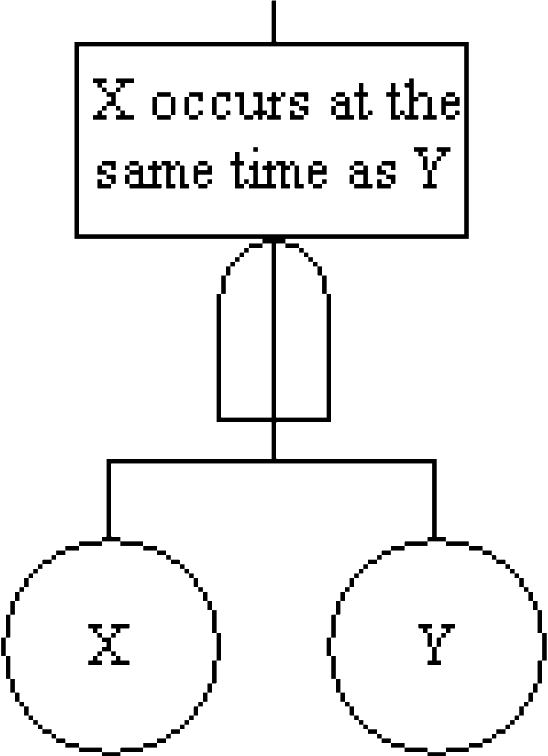
\includegraphics[height=4cm]{sand-walker}
\end{itemize}
\end{frame}

